\documentclass[11pt]{scrartcl}
\usepackage[utf8]{inputenc} % Kodierung der Textdatei mit Sonderzeichen
\usepackage[ngerman]{babel} % Sprache fuer Inhaltsverzeichnis etc.
\usepackage{amssymb} % Mathematische Symbole
\usepackage{amsmath} % Mehr mathematische Konstrukte
\usepackage{graphicx} % Um Bilder einbinden zu koennen
\usepackage{float} % fuer \begin{figure}[H]
\usepackage{icomma} % laesst das Komma als Dezimaltrennzeichen interpretieren
\usepackage{fix-cm} % für die große Titelschrift
\usepackage[pdftex]{hyperref} % Hyperlinks im Dokument
\hypersetup{colorlinks=true, linkcolor=black, citecolor=black, filecolor=black, urlcolor=black, pdftitle={LED-Spektrometer - Projektpraktikum 09/10 Gruppe 5}}


\newcommand{\unit}[1]{\ensuremath{\,\mathrm{#1}}} % Einheiten schreiben sich immer aufrecht!
\newcommand{\degr}{\ensuremath{^\circ}}
\newcommand{\cel}{\ensuremath{\degr\mathrm{C}}}
\newcommand{\dif}{\ensuremath{\mathrm{d}}}
\newcommand{\pdif}[2]{\ensuremath{\frac{\partial#1}{\partial#2}}}
\newcommand{\ee}[1]{\ensuremath{\cdot 10^{#1}}}
\newcommand{\hypref}[2]{\hyperref[#2]{{#1}~\ref{#2}}}

\setlength{\parindent}{1em}
\setlength{\parskip}{0.5\baselineskip}


\title{Direkte Messung der Erdrotation - Gruppe 5 WS 09/10, Projektpraktikum der Uni Erlangen}
\date{07.12.2009 -- 15.01.2010}
\author{Michele Collodo, Andreas Glossner, Karl-Christoph G\"odel, Bastian Hacker, Maria Obst, Alexander Wagner, David Winnekens}



\begin{document}
\sloppy % laesst Latex nicht ueber den Rand rausschreiben
\thispagestyle{empty}
\large{Projektpraktikum WS 09/10}
\hfill
\raisebox{-1.4cm}{
\includegraphics[width=5cm]{images/fau.pdf}}
\\[8\baselineskip]
\begin{center}
{\fontsize{36}{54}\textbf{Direkte Messung der Erdrotation}}
\\[2\baselineskip]
{\Large 07.12.2009 -- 15.01.2010}
\\[7\baselineskip]
{\huge\textbf{PPG 5}}
\\[0.5\baselineskip]
{\large\textbf{
Michele Collodo,
Andreas Glossner,\\
Karl-Christoph G\"odel,
Bastian Hacker,\\
Maria Obst,
Alexander Wagner,
David Winnekens}\\
Tutor: Xiaoyue Jin}
\vfill



\small{\url{http://pp.physik.uni-erlangen.de/groups/ws0910/ppg5/ppg5\_start.html}}
\end{center}
\newpage



\tableofcontents
\vfill



\begin{abstract}
Bla Abstract Bla
\end{abstract}
\newpage

\section{Einleitung} %Michele
Messung der Erdrotation - eines der \"altesten Experimente der Physik
\section{Grundprinzip - Tr\"agheitsmoment}

\begin{figure}[ht]
\begin{center}
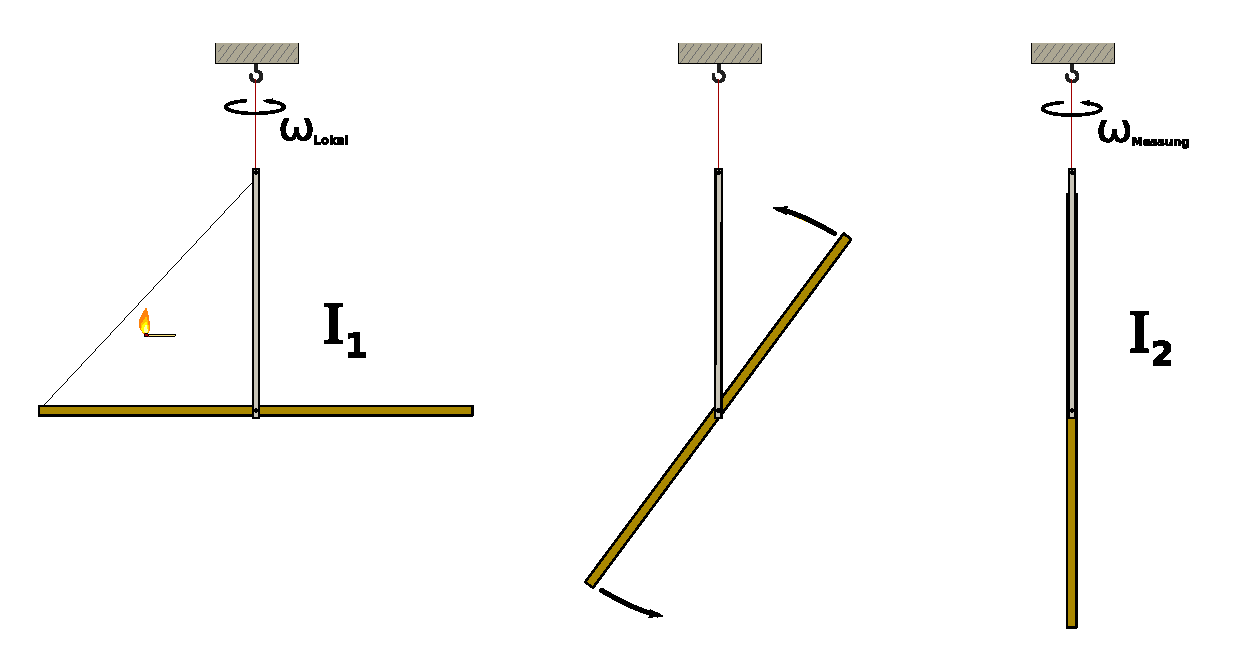
\includegraphics[width=0.8\textwidth]{images/prinzip.pdf}
\end{center}
\vspace{-1.5\baselineskip}
\caption{Schema des Bewegungsablaufs}
\label{prinzip}
\end{figure}

\section{Bau des Drehstabs} %Maria (solltest du nicht zu allem was wissen, sag bescheid)
\subsection{Material}
Magnetismus, Verwindung usw.
\subsection{Aufh\"angung}
Stabilisierung der Drehbewegung
\subsection{Klappmechanismus}
Zugmechanismus, Einrasten

\begin{figure}[ht]
\begin{center}
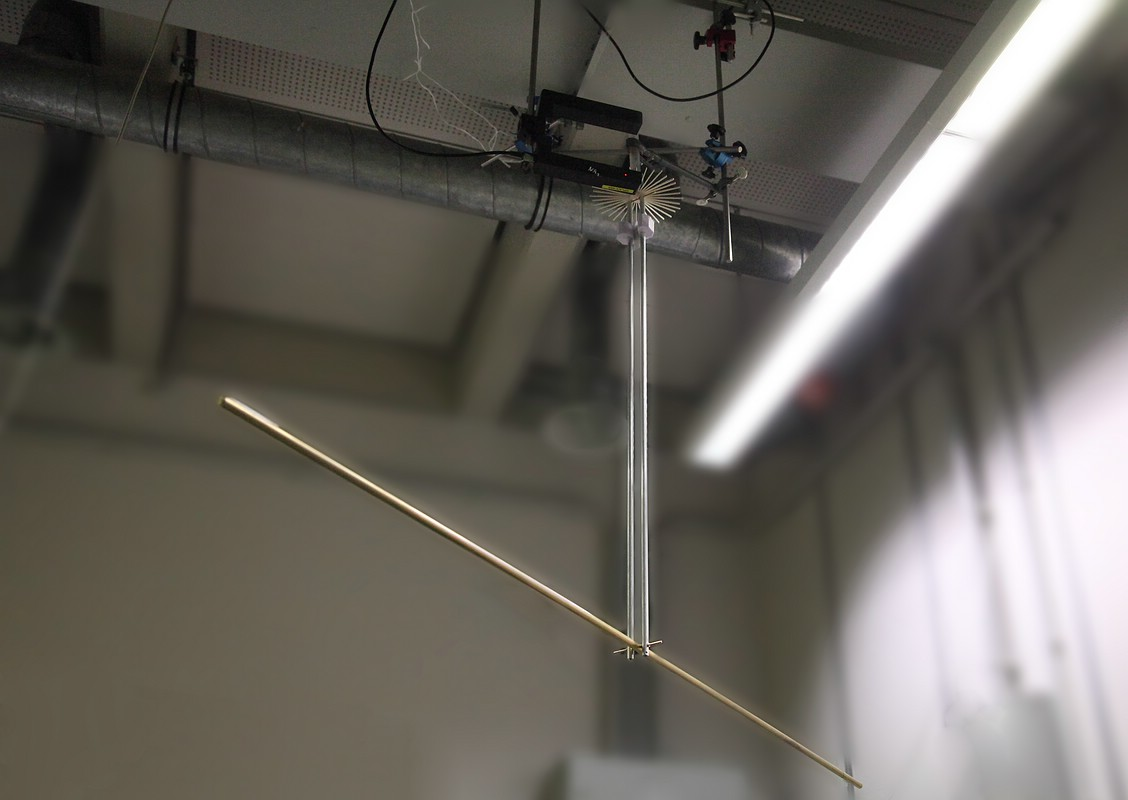
\includegraphics[width=0.8\textwidth]{images/stab-fertig.jpg}
\end{center}
\vspace{-1.5\baselineskip}
\caption{Der ausgelenkte Stab}
\label{stab-fertig}
\end{figure}

\section{Messungen}
\subsection{Berechnungen im Vorraus} %Andi
Tr\"agheitsmoment Rechnungen von Andi

\begin{figure}[ht]
\begin{center}
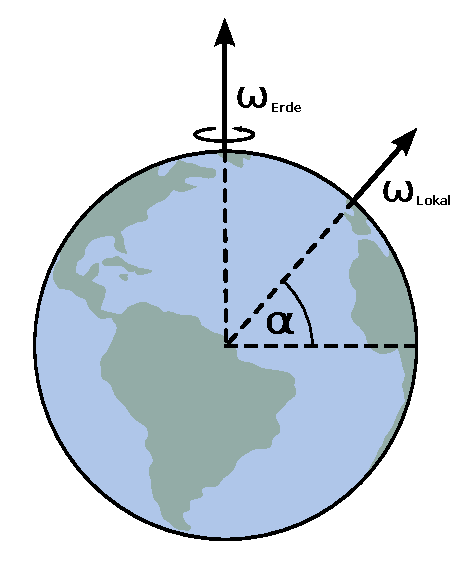
\includegraphics[width=0.2\textwidth]{images/welt.pdf}
\end{center}
\vspace{-1.5\baselineskip}
\caption{Position auf der Welt}
\label{Welt}
\end{figure}

\subsection{Cassymessungen} %Axi
Zur Aufzeichnung der Drehung des Stabes kam zun\"achst das CASSY Lab System zum Einsatz. Auf der H\"ohe der Spitze des Stabes wurde eine Lichtschranke durch Stativstangen an der Deckenkonstruktion verschraubt, welche die Durchg\"ange des Stabes z\"ahlte. Die Ausl\"osung der Lichtschranke sollte durch einen leichten Querstab aus Balsaholz erfolgen. Es stellte sich jedoch heraus, dass dabei nur unzureichende Genauigkeiten bei der Ermittlung der Drehgeschwindikeit erzielt werden konnten, da die Lichtschranke bei dieser Methode nur zweimal pro ganzer Umdrehung ausgel\"ost wird. Deshalb wurde an der Spitze des Stabes ein \glqq Speichenrad\grqq installiert. Die einzelnen Speichen hatten dabei einen Abstand von jeweils $10$. Pro Umdrehung wurde die Schranke also 36 Mal ausgel\"ost. Die L\"ange der Speichen wurde so kurz wie m\"oglich gehalten um das Tr\"agheitsmoment des Stabes nicht unn\"otig zu beeinflussen.

\begin{figure}[h]
\begin{center}
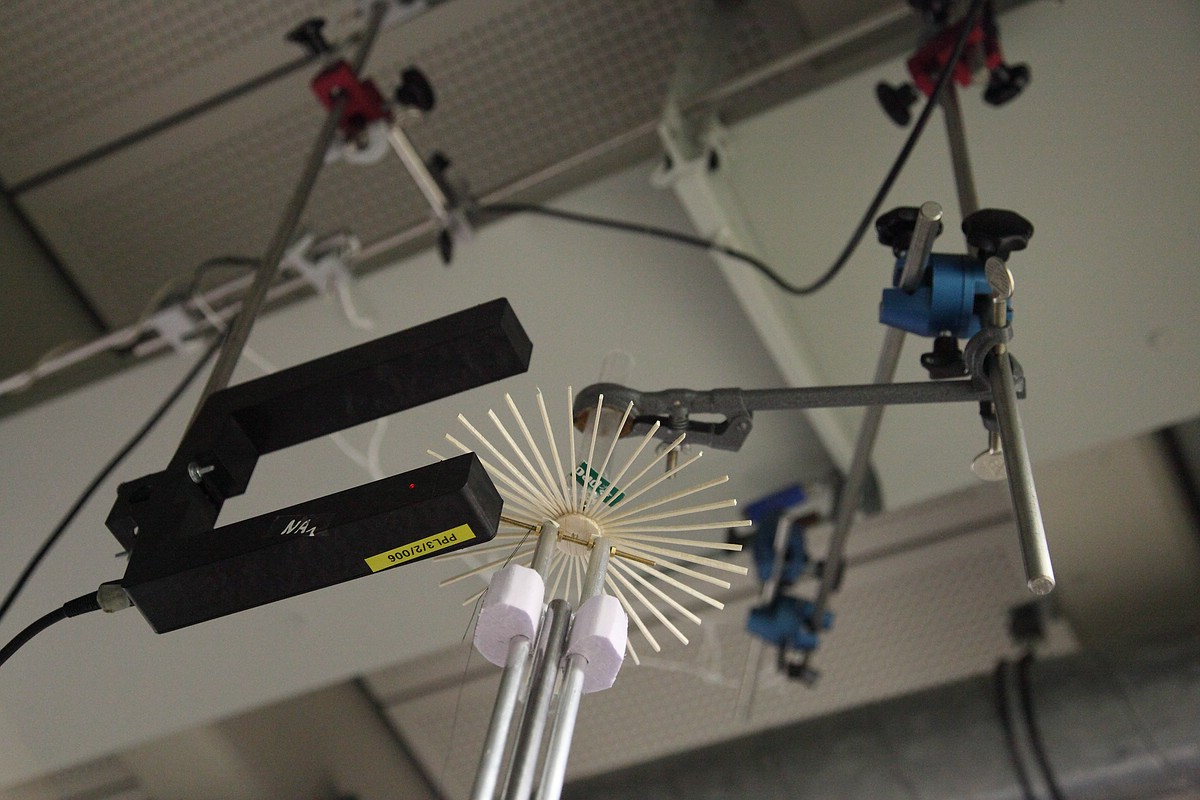
\includegraphics[width=0.8\textwidth]{images/lichtschranke.jpg}
\end{center}
\vspace{-1.5\baselineskip}
\caption{Das Speichenrad beim Durchgang durch die Lichtschranke}
\label{lichtschranke}
\end{figure}

\subsection{Videomessungen} %Karl


\section{Verbesserungsvorschläge} %David faden, zwei stäbe, kamera von oben, symmetrischerer aufbau


\section{Fazit} %Basti
Nicht alles funktioniert so, wie erwartet \dots $\rightarrow$ Warum?

\end{document}
